\documentclass[11pt, a4paper]{article}		% general format


%%%% Charset
\usepackage[utf8]{inputenc}					% use utf8					
\usepackage[russian]{babel}					% use russian font


%%%% Math
\usepackage{amsmath}						% Amer­i­can Math­e­mat­i­cal So­ci­ety (AMS) math fa­cil­i­ties
\usepackage{amsfonts}						% fonts from the AMS
\usepackage{amssymb}						% additional math symbols


%%%% Graphics
\usepackage{graphicx}


\author{Дедков Сергей}
\title{Отчет по лабораторной работе №1 :\\ \LaTeX{}, Git, GPG}
\date{2015}

%---------------------------------------------------------

\begin{document}
\maketitle
\tableofcontents
\newpage

%---------------------------------------------------------


\section{Цель работы}

Определить набор и версии сервисов запущенных на компьютере в диапазоне адресов.
Данная работа выполняется на ОС kali linux, используется утилита nmap.



%---------------------------------------------------------

\section{Ход работы}


%---------------------------------------------------------

\subsection{Провести поиск активных хостов}

Выполним поиск в подсети 192.168.76.0/24. Для этого воспользуемся командой nmap 192.168.76.0/24.
В результате видим 5 хостов, один из них - виртуальная машина с запущенной metasploit, а именно с ip адресом 192.168.76.136.

\begin{figure}[h!]
\centering
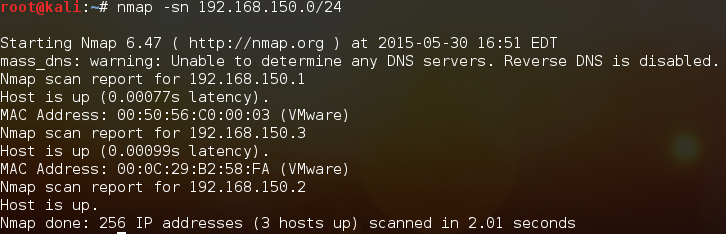
\includegraphics[scale=0.68]{res/hosts_search}
\caption{Поиск хостов}
\end{figure}

\end{document}